\title{Trending topics using the Twitter-API}
\author{
        Marco Pock-Steen Fraile \\
        Christian Palmh\o j Nielsen \\
        IT University of Copenhagen\\
}
\date{\today}

\documentclass[12pt]{article}

\usepackage{graphicx}

\begin{document}
\maketitle

\begin{abstract}
We have designed an algorithm for identifying trending topics in twitter..
\end{abstract}

\section{Introduction}
We wish to make use of the Twitter streaming API to implement our own version of trending topics using the Misra-Gries algorithm, and for the trending topics we would track how many unique tweets have been made per topic, using one of the algorithms for counting distinct elements. We could also count number of tweets for trending topics to compare actual tweets with unique tweets, but this is not algorithmically a challenge.
\newline\newline
Challenges would include finding a suitable k for the Misra-Gries that is a good trade-off between memory space and making sure we take into account the tweets inbetween the actual trending topics that might "flood" them out of the array.
\newline\newline
For the counting algorithm we similarly need to find a good hashing algorithm for tweets, and based on this find a good number for kth-minimum distances that gives us a realistic count for unique tweets.

\paragraph{Outline}
The remainder of this article is organized as follows.
Section~\ref{related work} gives account of previous work.
Our new and exciting results are described in Section~\ref{results}.
Finally, Section~\ref{conclusions} gives the conclusions.

\section{Twitter topics}
Twitter is a real-time information network that connects you to the latest stories, ideas, opinions and news about what you find interesting.

At the heart of Twitter are small bursts of information called Tweets. Each Tweet is 140 characters long. An example of a tweet can be seen below.
\newline

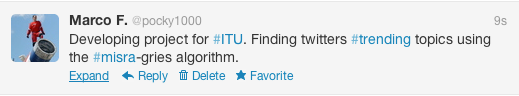
\includegraphics[width=125mm]{tweet.png}

Users of twitter can see the tweets of people they follow, and have the options to either reply to a tweet, or retweet it. On retweet the user basically shares the same message to their own followers, giving credit to the creator of the message.
The topic of a tweet is identified by the presence of a hashtag \# in front of a word. In the example above the topics are \#ITU,\#trending and \#Misra.
Tweets can be tagged by writing a hashtag "\#" followed by a topic or keyword. Twitter users this as a way to categorize messages.
A trending topic is defined by a topic that has a high frequency, in other words many people are "tweeting" about the same topic at some point in time. A trending topic can either be many unique tweets about the same topic, e.g. if people are tweeting to promote some beneficial cause, or it can be the same message retweeted by many users.
Twitter currently have over 500 million users, so the amount of tweets produced at any moment is equally big, some specifics. We use the public Twitter API to create a stream of which corresponds to a sample of all tweets. 

\section{Streaming algorithms}\label{related work}
\subsection{Heavy hitters}
\subsection{Misra-Gries}

\section{Algorithm design}

\subsection{Data structure}
When a new tweet is registered the algorithm has to determine if the contained topic has already been seen. We need a data structure that provides fast lookup, such as a dictionary with key-value pair as topic-frequency. We also need to find a data structure that allows for decrementing all values by 1 if the topic is not already created. Lastly we will have to find a way to randomly remove a topic if the data structure exceeds k at the creation of a new topic.
\subsection{Design}
\subsection{Running time}
\subsection{Satisfiability}

\section{Results}\label{results}
In this section we describe the results.

\section{Conclusions}\label{conclusions}
We worked hard, and achieved very little.

\bibliographystyle{abbrv}
\bibliography{simple}

\end{document}
This is never printed